\chapter{INTRODUCTION}
\label{chp:1}
\section{Global Renewable Energy Status}
\begin{figure}[h]
	\centering
	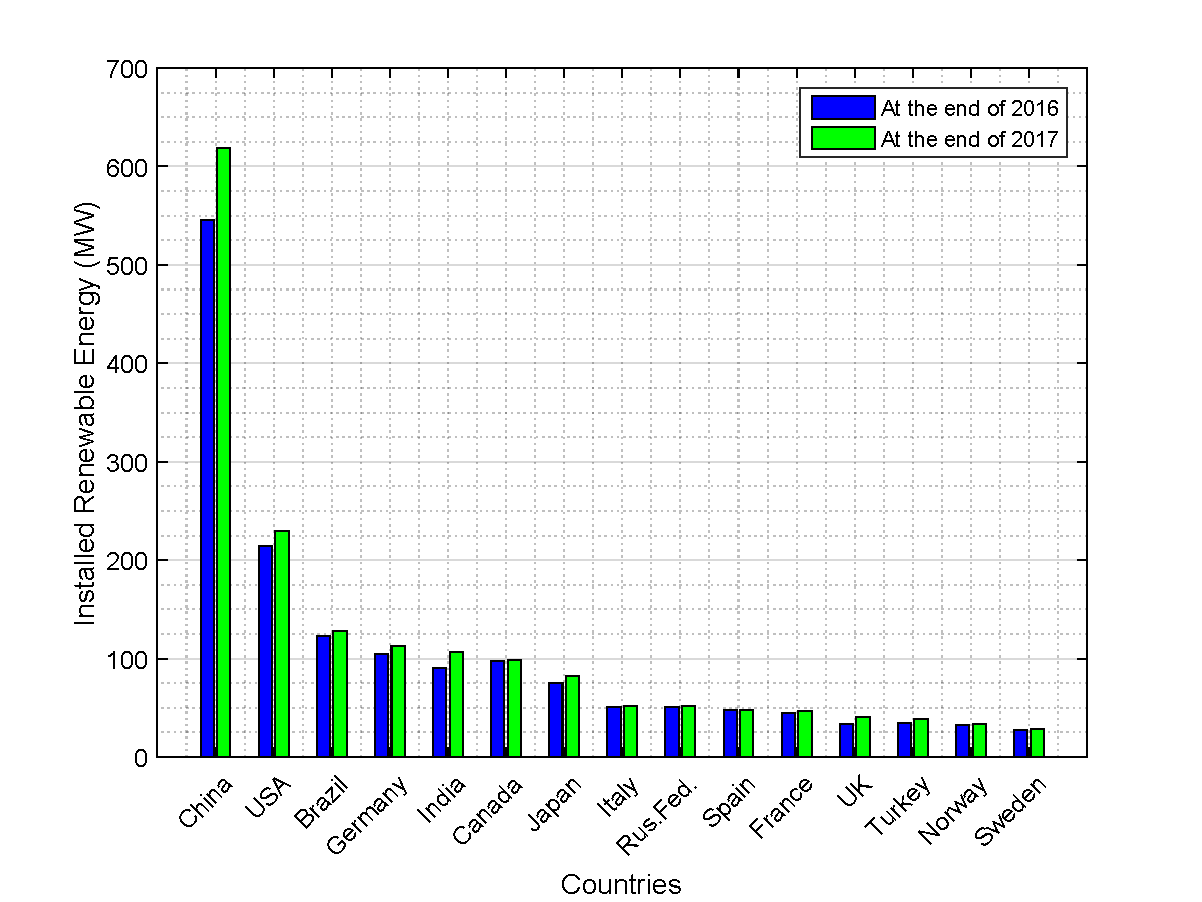
\includegraphics[scale=0.7]{renewablecapacities.pdf}
	\caption{Installed Renewable Energy Capacity of Leading Countries}
	\label{renewablecap}
\end{figure}
Renewable energy is still one of the hottest topics in the power area. The share of the renewable energy systems has been reached significant levels. At the end of 2017, the renewable power capacity has reached 2179 GW throughout the world including hydro power plants \cite{InternationalRenewableEnergyAgencyIRENA2018}. Fig. \ref{renewablecap} shows the installed renewable energy capacity for leading countries at the end of 2016 and 2017 \cite{InternationalRenewableEnergyAgency2017}, \cite{InternationalRenewableEnergyAgencyIRENA2018}. China, USA, Brazil and Germany constitutes almost half of the world total capacity. China has the biggest installed renewable capacity so far and increased its capacity by 73 GW in 2017 which is very close to the whole installed electrical power of the Turkey. This indicates the severity of the growing renewable demand.\par
\begin{figure}[h]
	\centering
	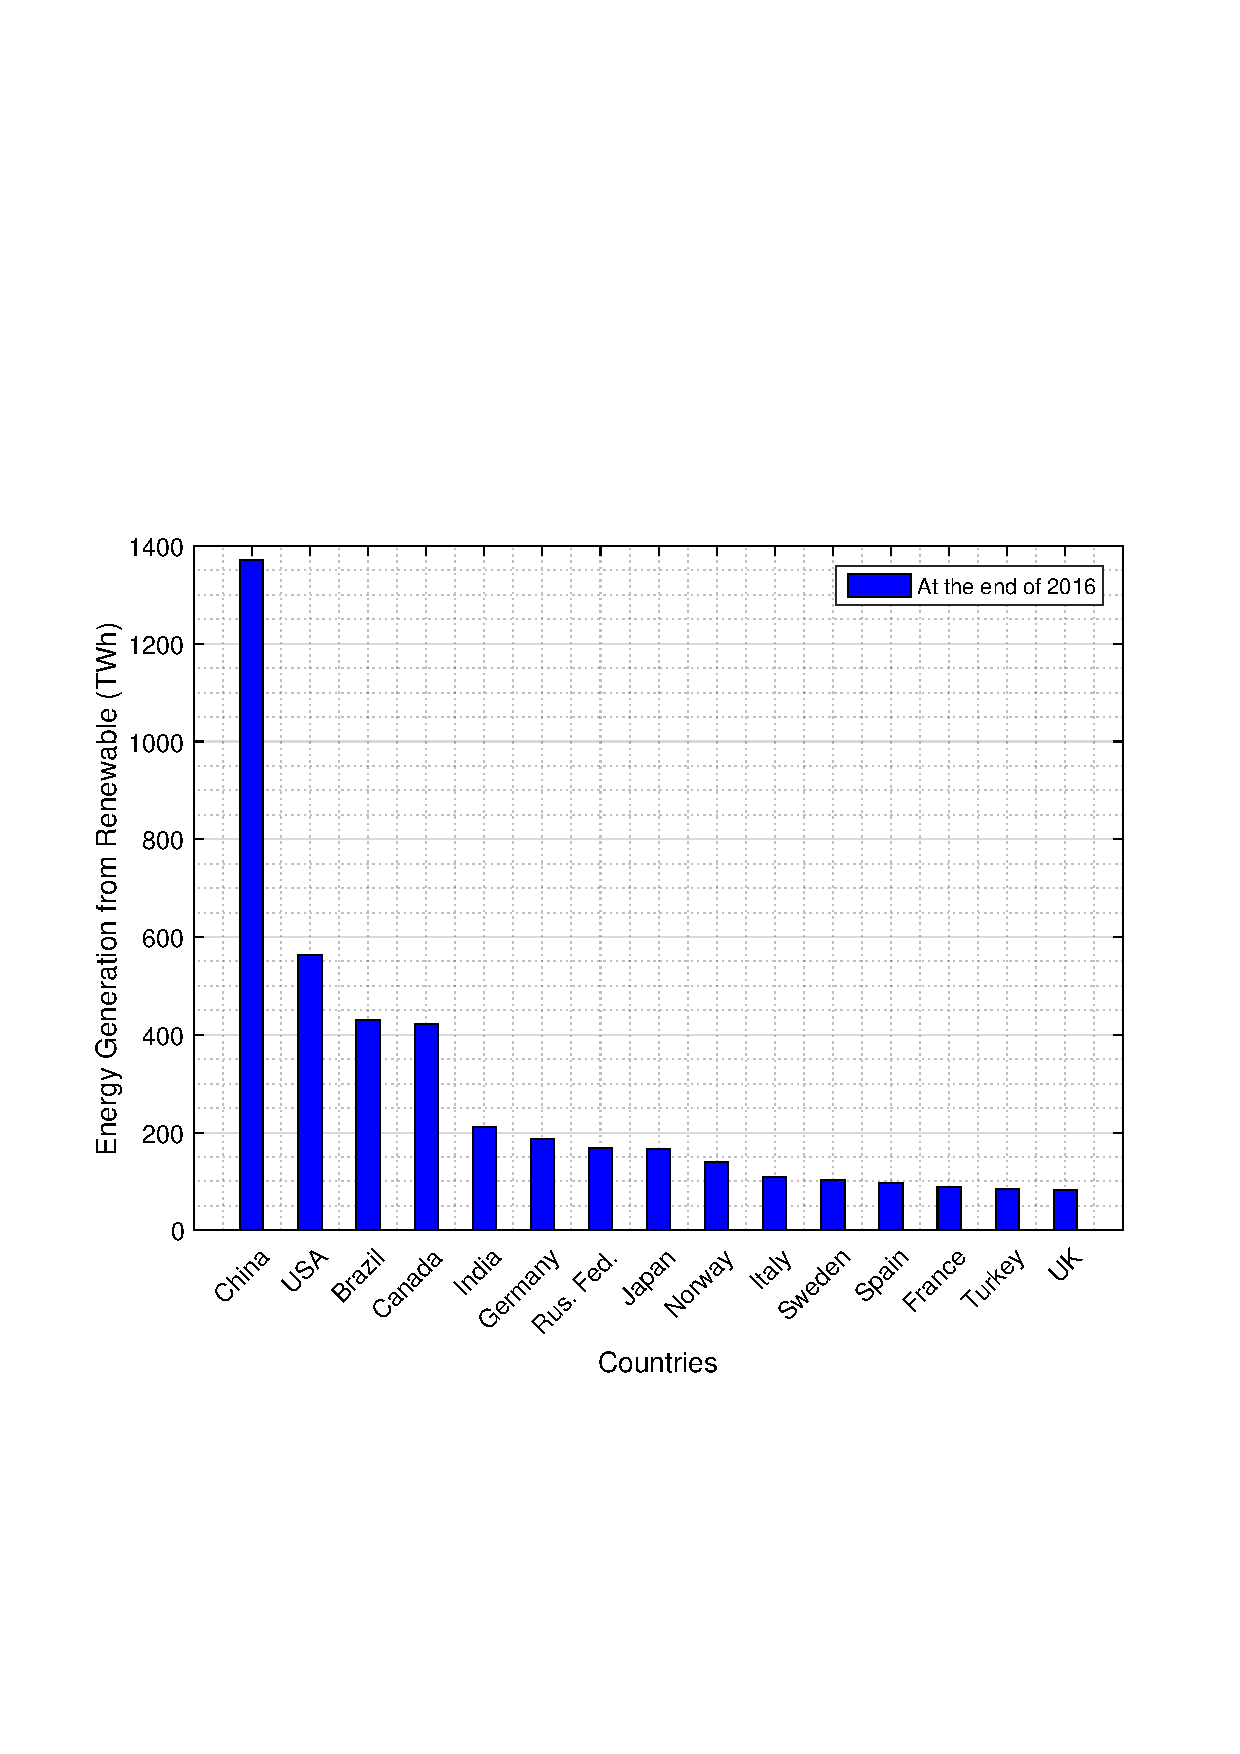
\includegraphics[scale=0.7]{renewableproduction.pdf}
	\caption{Renewable Energy Production of Leading Countries}
	\label{renewablepro}
\end{figure}
Fig. \ref{renewablepro} shows the energy production from renewable energy  systems {InternationalRenewableEnergyAgency2017}. It is obvious that China, USA and Brazil produces highest amount of energy from renewable since they already have the highest installed capacity. However, India and Canada produces more energy than Germany even though Germany has more installed renewable capacity. This result is due to the fact that renewable energy production is dependent on parameters such as solar radiation and wind speed depending on the renewable source. This can be better observed in Fig. \ref{production/capacity} which shows the average energy generation from per MW renewable energy sources  in 2016 \cite{InternationalRenewableEnergyAgency2017}. For a MW renewable energy system, Germany produces the lowest amount of energy meanwhile Canada and Norway produce highest amount among these countries. Turkey has one of the lowest installed capacity and energy generation from renewable systems among the listed countries. However, it is listed in the middle of these countries due to its high potential for renewable energy systems.
\begin{figure}[h!]
	\centering
	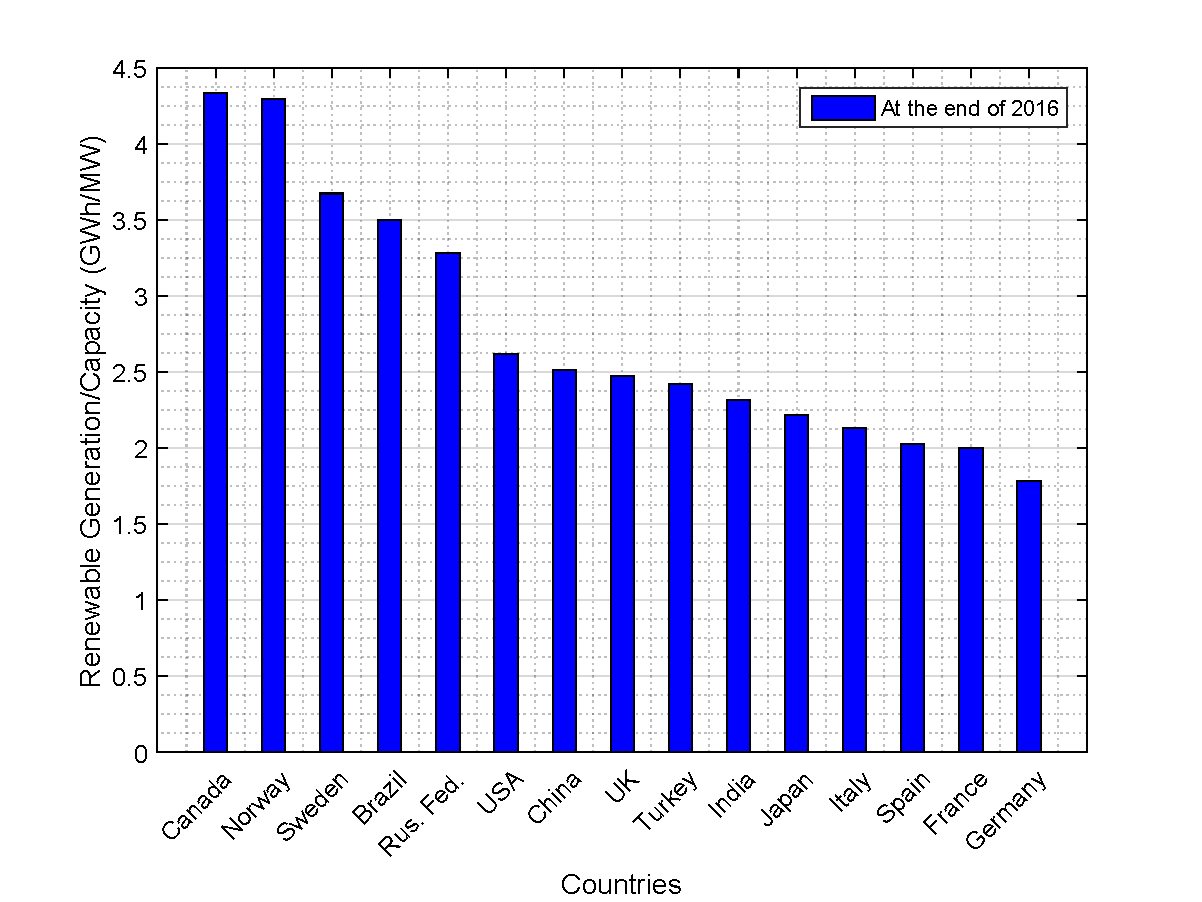
\includegraphics[scale=0.7]{renewablepro_cap.pdf}
	\caption{Average Renewable Energy Generation per MW in 2016}
	\label{production/capacity}
\end{figure}
\subsection{EU 2020 Goals}
In 2008, 20 20 by 2020-Europe's Climate Change Opportunity report has been released by EU Commission and two key targets are set for 2020 \cite{EuropeanCommission2008}: 
\begin{itemize}  
	\item At least 20 \% reduction in greenhouse gases (GHG) by 2020
	\item Achieving 20\% renewable energy share in energy consumption of EU by 2020
\end{itemize}
The Renewable Energy Directive is published in 23 April 2009. This directive has set national binding targets for EU countries in order to accomplish the 20\% renewable energy target for EU and 10 \% target for the renewable energy usage in the transport. \cite{EuropeanParliament2009} As a result, each EU country has been determined their national action plans. In order to achieve the 20 \% target, each member state determine their own targets ranging from 10\% in Malta to 49\% in Sweeden. According to the latest release by Eurostat, renewable share of the EU in energy consumption has reached 17 \% in 2016 \cite{States2016}. Moreover, eleven of EU member states has already achieved their 2020 targets. Renewable shares of EU members are shown in Figure \ref{EUtargets}.
\begin{figure}[h!]
	\centering
	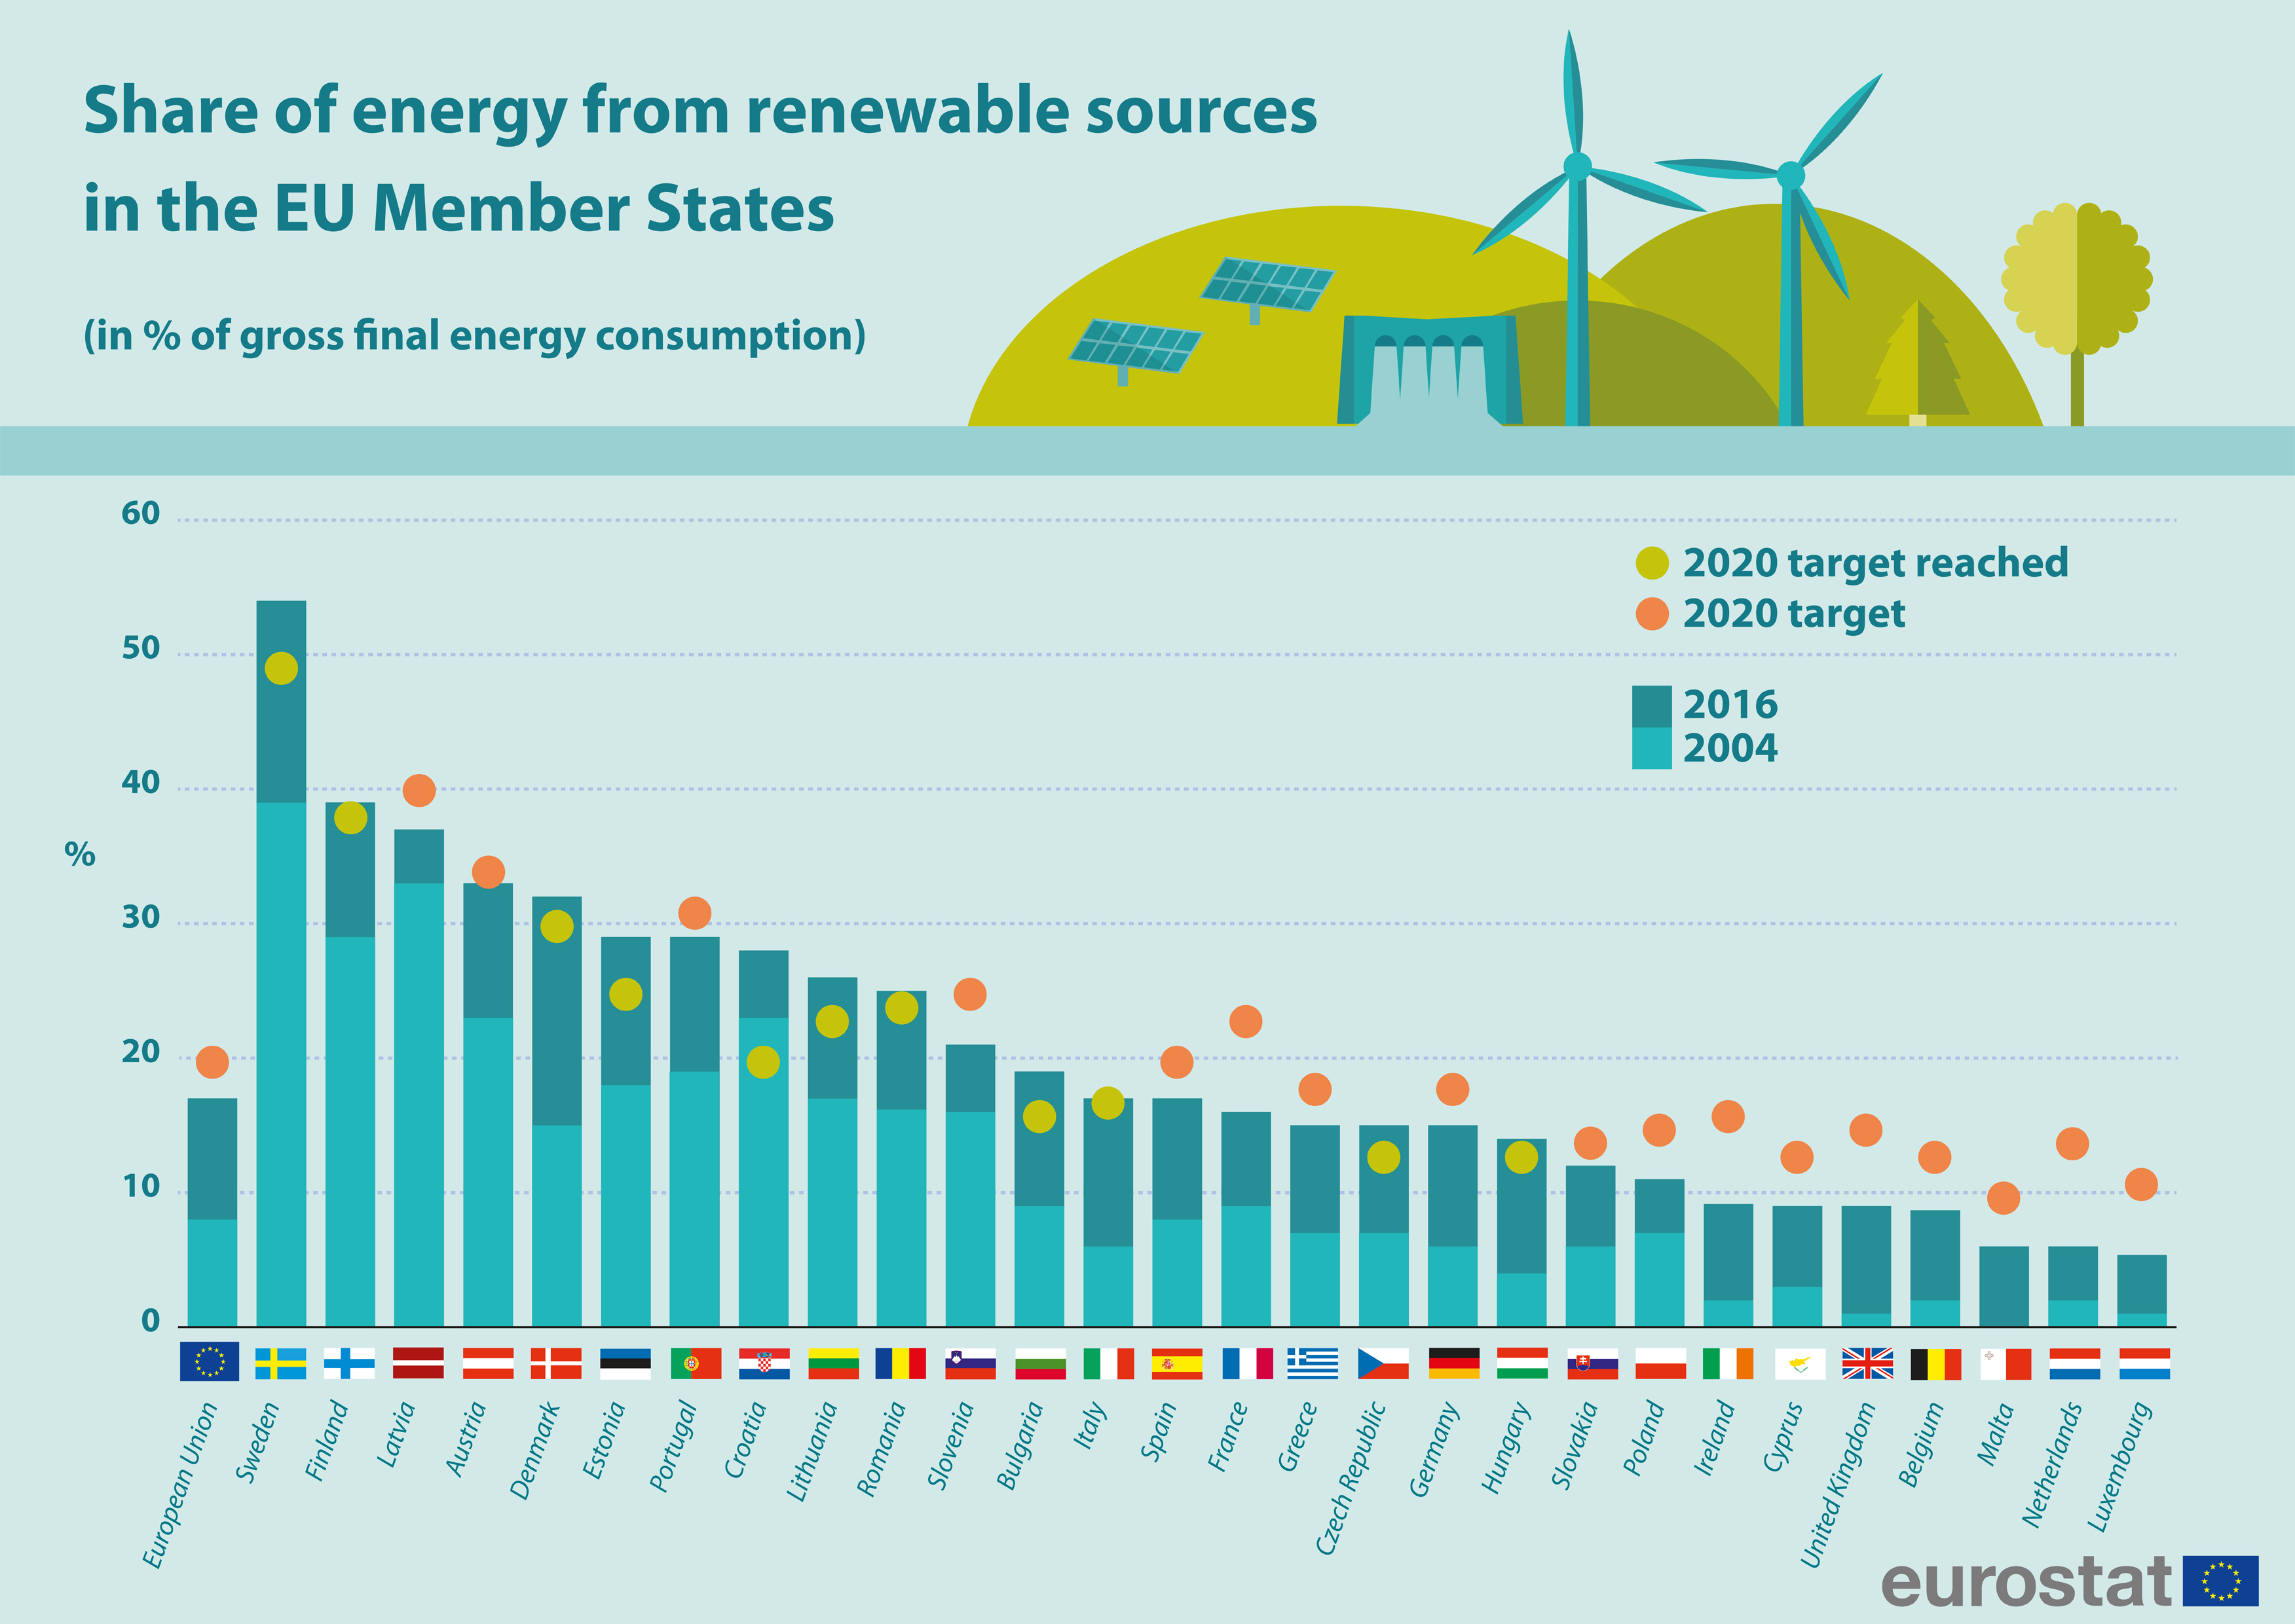
\includegraphics[scale=0.11]{Figure_1-Share_of_energy_from_renewable_sources_2004-2016.png}
	\caption{Renewable Targets of EU Member States\cite{States2016}}
	\label{EUtargets}
\end{figure}
\subsection{Wind Energy Status}
Wind power has the highest share in the installed renewable energy capacity except for hydro power. The wind power capacity at the end of 2017 has reached 514 GW worldwide\cite{InternationalRenewableEnergyAgencyIRENA2018}. The wind power capacity of the leading countries is shown in the Fig. \ref{windcap}. As in the case of total installed renewable energy capacity, China and USA have also the highest installed capacities in the wind power capacity. \par
\begin{figure}[h!]
	\centering
	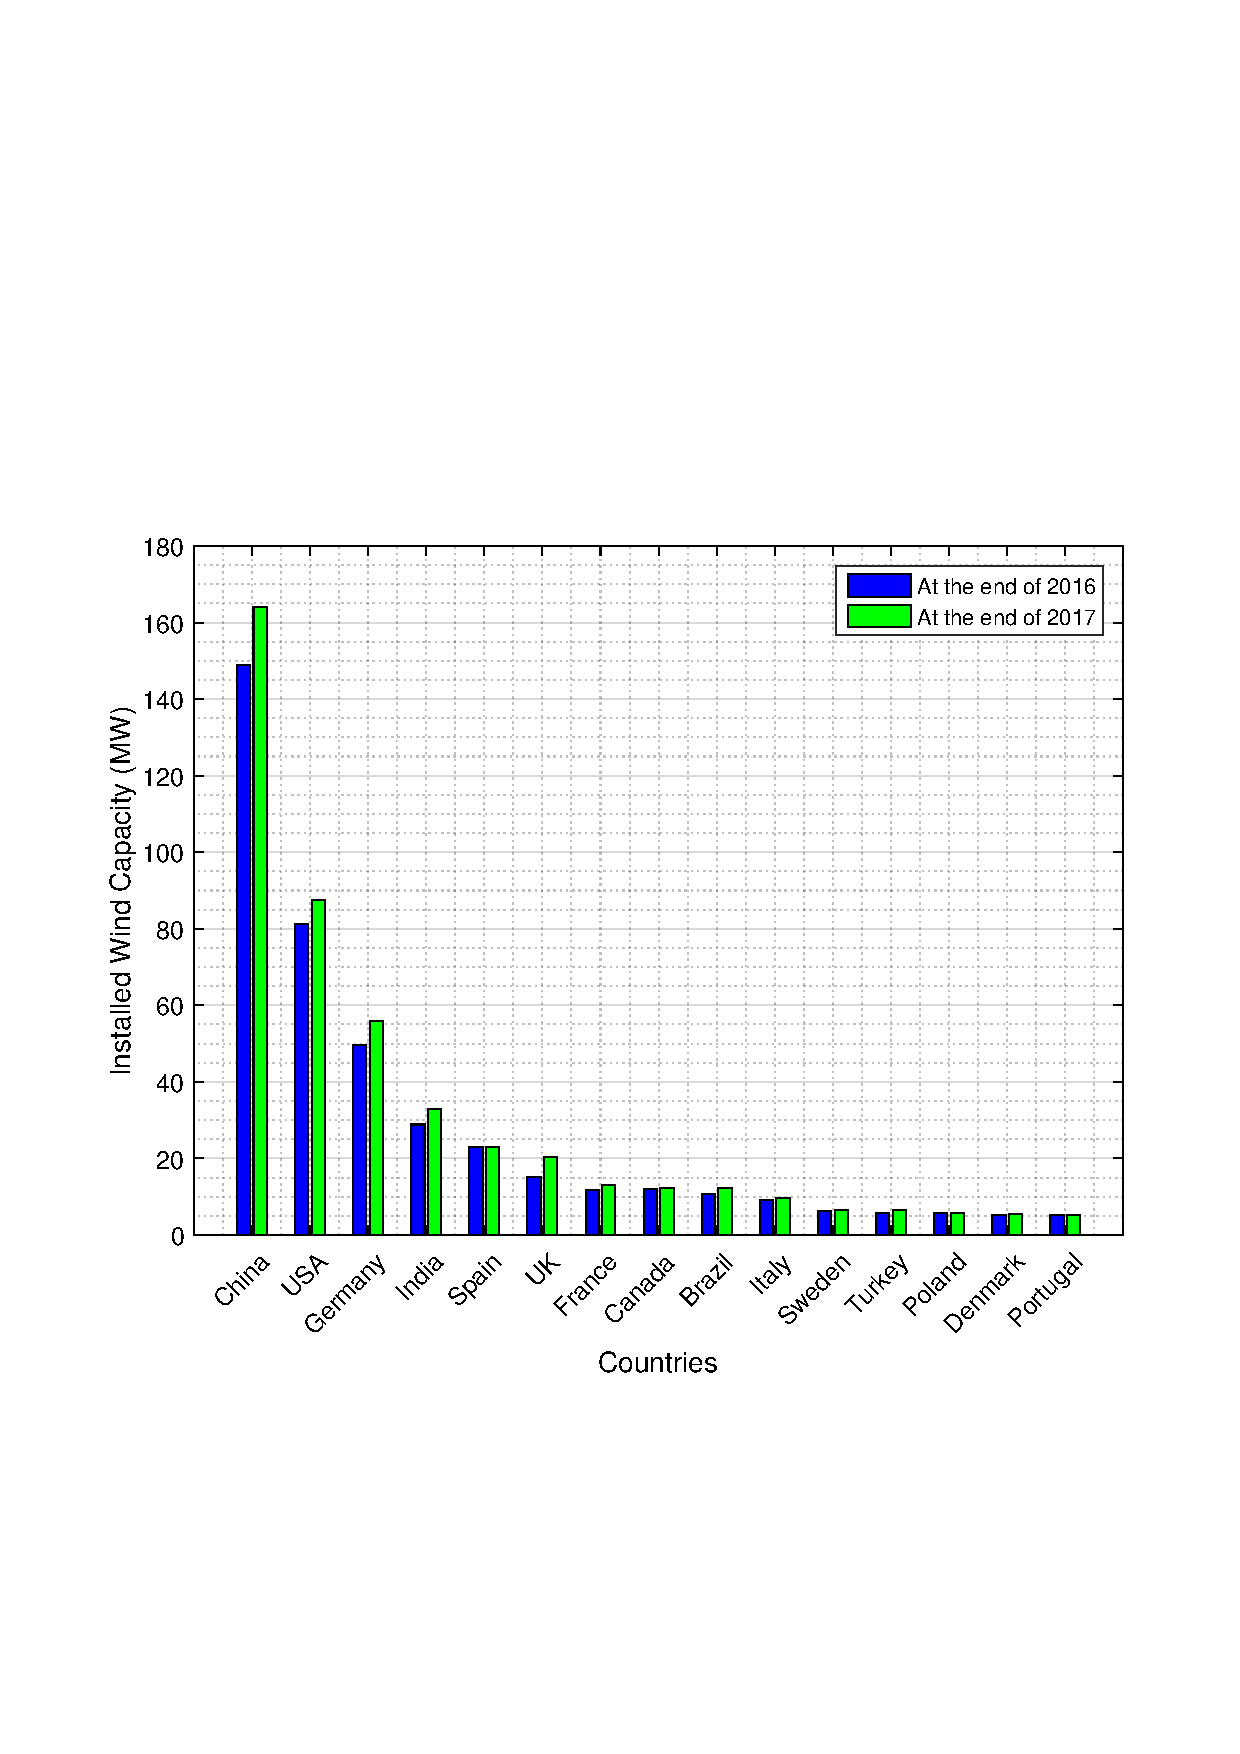
\includegraphics[scale=0.7]{windcapacity.pdf}
	\caption{Wind Power Capacity of Leading Countries in 2016}
	\label{windcap}
\end{figure}
The energy production from wind energy is shown in the Fig. \ref{windpro}. Even though China has the highest wind power capacity,  USA generates highest amount of energy from wind. The energy production per a MW wind energy system is shown in the Fig. \ref{windpro_cap}. Denmark, UK and Sweden yield highest energy from per MW wind energy system due to its wind potential meanwhile Germany, India and China generates minimum energy.
\begin{figure}[h!]
	\centering
	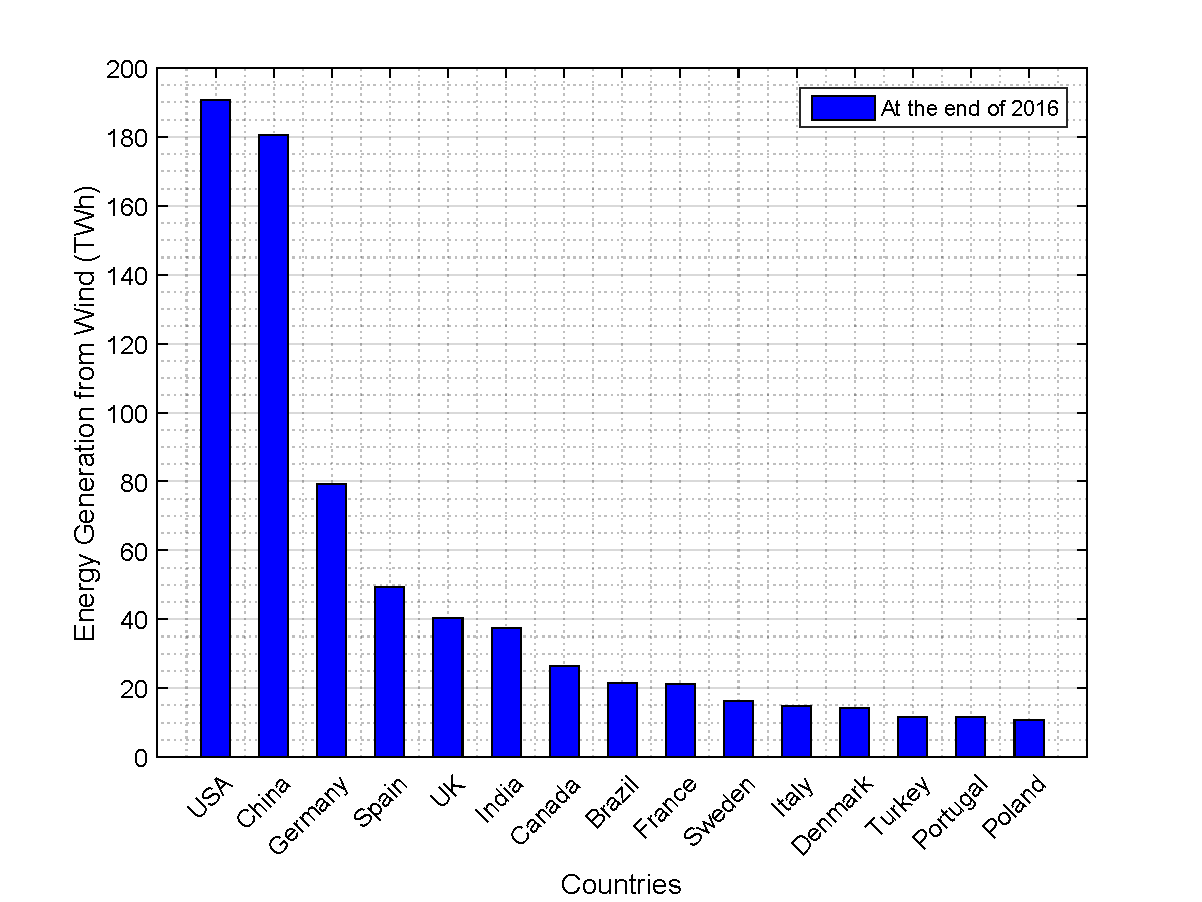
\includegraphics[scale=0.7]{windproduction.pdf}
	\caption{Wind Power Production of Leading Countries in 2016}
	\label{windpro}
\end{figure}
\begin{figure}[h!]
	\centering
	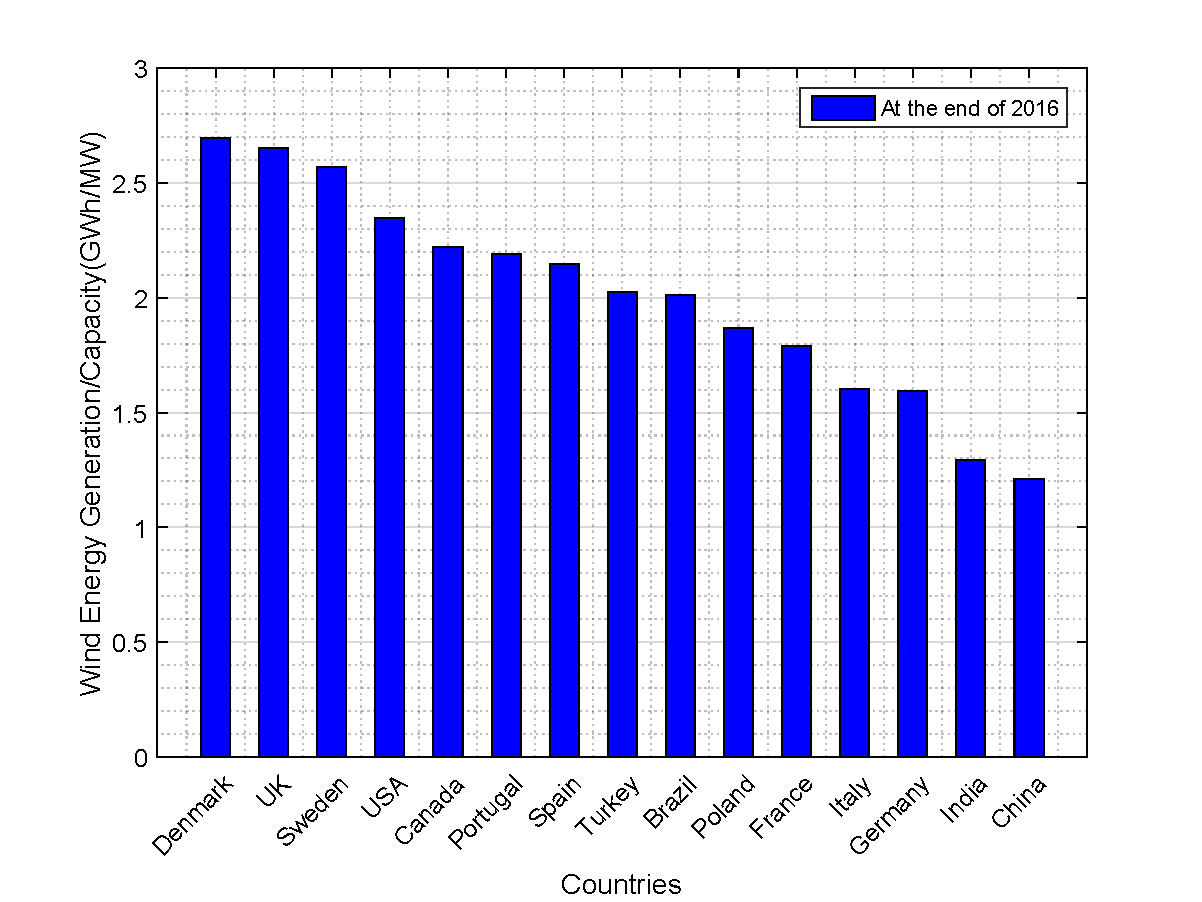
\includegraphics[scale=0.7]{windpro_cap.pdf}
	\caption{Wind Power Production of Leading Countries in 2016}
	\label{windpro_cap}
\end{figure}

\section{Global Renewable Energy Future}
The share of renewable energy is increasing each passing day. Today, reports arguing the possibility of even 100\% renewable energy region by region is published\cite{REN212017d}. The renewable energy reports estimate the share of renewable energy in the total energy consumption for 2030 and 2050. Figure \ref{EU2030} shows the EU renewable energy share for 2030. Moreover, the report published by IRENA (International Renewable Energy Agency) estimates the share of renewable energy in EU as 24\% by 2030 which is below proposed target of 27\%\cite{IRENA2014}.\par
\begin{figure}[h!]
	\centering
	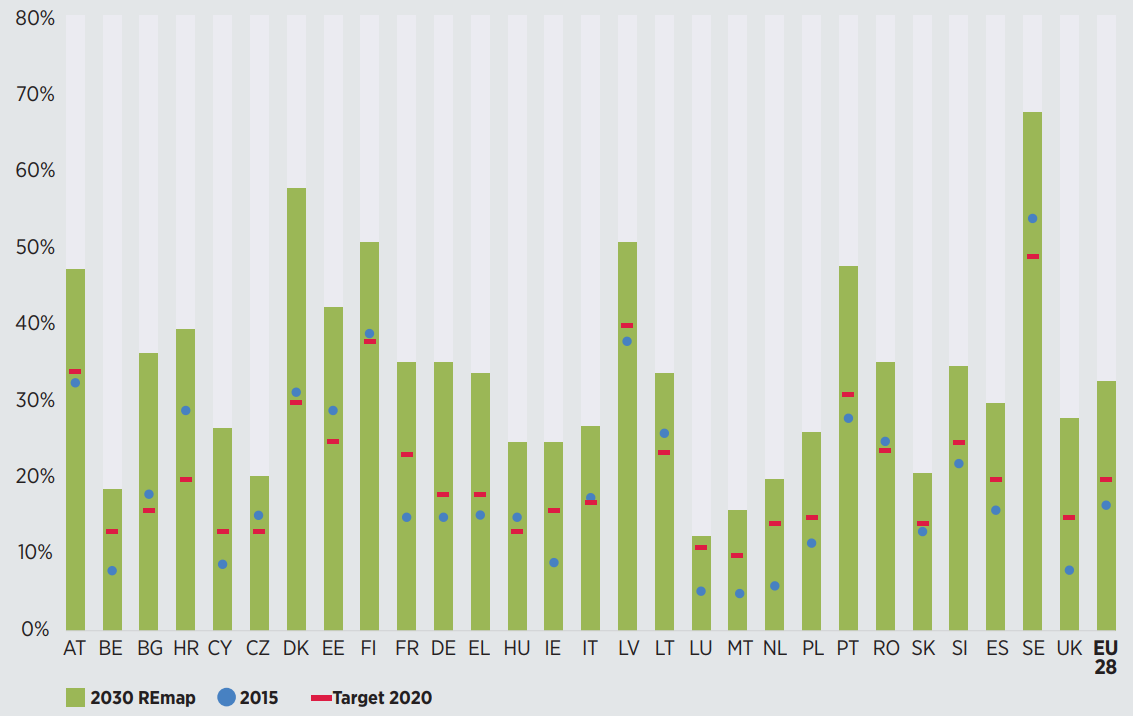
\includegraphics[scale=0.35]{EU2030.png}
	\caption{Renewable energy share in total energy consumption by EU for 2015, 2020 targets and 2030 potential according to REmap \cite{EuropeanCommission2018}}
	\label{EU2030}
\end{figure}
\begin{figure}[h!]
	\centering
	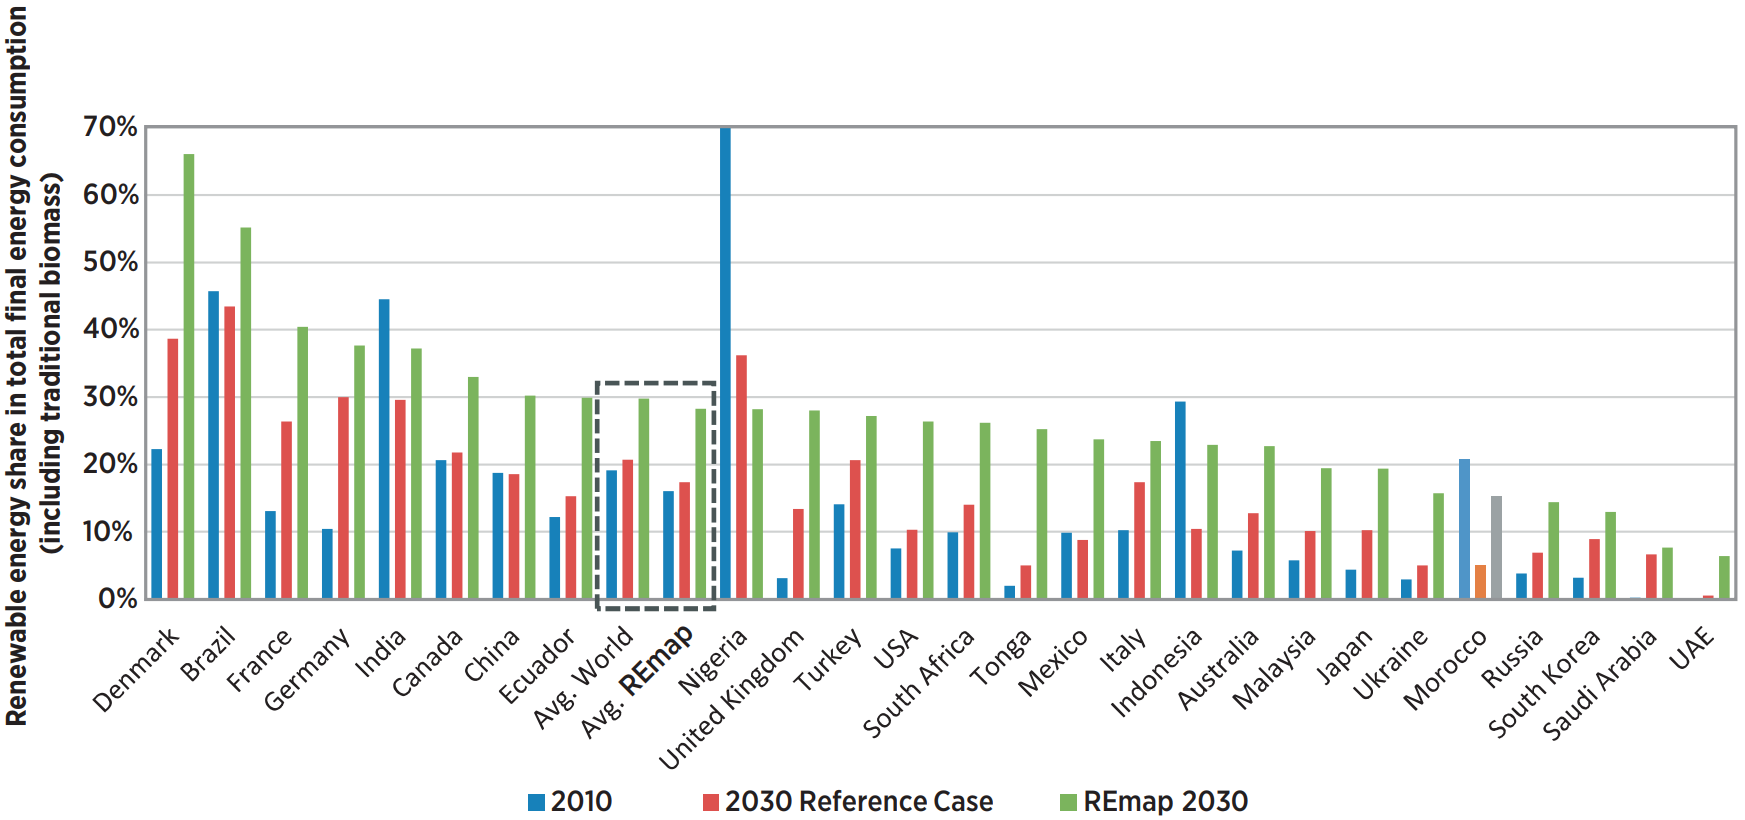
\includegraphics[scale=0.3]{2030map2.png}
	\caption{Renewable energy shares for 2010, 2030 Reference Case and 2030REmap \cite{IRENA2014}}
	\label{2030map}
\end{figure}
Renewable shares of REmap countries in 2010, 2030 reference case and 2030REmap and the world average are also shown in Fig.\ref{2030map}. The only country whose renewable energy decreases in the 2030 is Nigeria. The reason is that the main source of energy in Nigeria is biogas for the time being. However, the renewable share is expected to decrease dramatically as the industry switches to natural gas.
\section{Renewable Energy Problems}
It is an undeniable fact that renewable energy systems are advantageous in terms of global warming and carbon dioxide emission. Nonetheless, they also have disadvantages to the system operators due to intermittent energy generation profile. First of all, the term intermittent in the literature is related to the variable and uncontrollable nature of the renewable sources \cite{KlingeJacobsen2010}. Since the source of the RES is variable, it is not possible to adjust its output according to the demand. Therefore, the thermal plants have to be in the operation when high wind speeds and solar radiation exist. Moreover, the system requires additional start-ups and rise from partly loaded plants in order to balance the energy in the system because of the uncertainty of RES. These all create additional costs caused by high share of RES in the system \cite{Zipf2013}. Moreover, power grid will face with transmission system issues as overloaded transmission lines, changes on the protection and control in the distribution system, greater level of power-factor control and low voltage ride-through (LVRT) requirements when the RES share is increased in the grid\cite{Ipakchi2009}.\par
Another challenge of increasing RES is the problem of power system frequency stability. Since the frequency of the power system depends on the balance between generation and consumption, grid operators are responsible for adjusting the generation in order to maintain a constant frequency. However, the renewable energy generation is strictly dependent on the renewable source i.e. solar radiation or wind speed. Therefore, renewable systems makes the system operation harder due to their intermittent and uncertain power generation profiles. Moreover, as the renewable systems with power electronics interface increase in the electricity grid, the grid equivalent inertia decreases. In \cite{Gautam2011}, the reduced grid inertia due to the high DFIG wind turbine penetration is emphasized. Moreover, the results of the reduced grid inertia following a disturbance is listed as: 
\begin{itemize}
	\item increased effective aggregated angular acceleration of synchronous machines which require high restoring forces
	\item high rate of change of frequency and hence, decreased frequency nadir
\end{itemize}
It should be noted that this problem is not specific to DFIG wind turbines but renewable energy systems which are connected to grid with power electronics. Conventional synchronous generators rotates with synchronous speed which is proportional to grid frequency. If the grid frequency decreases, then the synchronous speed also decreases. In this case, the generator active power is increased inherently due to kinetic energy extraction from the generator inertia. The increase in active power provides action time for primary controllers and crucial for frequency stability. Type-1 and Type-2 wind turbines are directly connected to grid. Hence, the frequency deviations affects the active power output of such wind turbines\cite{Muljadi2012}. Nonetheless, active power output of renewable energy systems with power electronics such as Type-3 and 4 wind turbines and photovoltaic systems is not affected from the grid frequency deviations. Therefore, these system have no contribution to the grid inertia whether the system includes inertia or not. Hence, the aggravated grid inertia is reduced with the penetration of RES. The comparison for different type of generators is made in \cite{VanDeVyver2016} and listed in Table \ref{generatorcomparison}.\par  
\begin{table}[h!]
	\centering
	\begin{tabular}{lc}
				\hline
		\multicolumn{1}{c}{\textbf{Type of the generator}}                                                                            & \textbf{Inertial Response Behaviour} \\ \hline
		Conventional Synchronous Generator                                                                                            & ++                                   \\
		Fixed Speed Induction Generator (FSIG)                                                                                        & +                                    \\
		Doubly Fed Induction Generator (DFIG)                                                                                         & -                                    \\
		\begin{tabular}[c]{@{}l@{}}Variable Speed Wind Turbine Generator\\ (Connected with Full Scale Power Electronics)\end{tabular} & None                                 \\ \hline
	\end{tabular}
	\caption{Comparison of Different Type of Generators for Inertial Response Behaviour}
	\label{generatorcomparison}
\end{table}
Another reason for the decrease in the grid inertia is the de-commitment or dispatch of the conventional sources due to economic concerns. Since the renewable energy has the lowest cost for energy production, it preferred instead of conventional generators. As a result, conventional generators are dispatched to a lower generation profile or taken-off from operation.\par
Note that grid inertia is directly related to the amount of load in the system in addition to the share of RES. Therefore, the amount of online generator flactuates within time. Hence, the scenario in which the system has low demand and also high renewable generation is the most critical one since the lowest grid inertia will be faced in the network.
\section{Literature Review}
Studies regarding inertial support date back to early 2000s. In the study \cite{Lalor2004}, the effect of the increasing wind energy penetration has been investigated. The study concludes that increasing share of wind energy increases the primary reserve requirement for the successful grid operation. The increased frequency deviations, especially in light load conditions (high wind generation with low consumption scenario) can be mitigated in the system as long as the wind generation provides inertia support. Study in \cite{Ekanayake2003} states that DFIG wind turbines are de-coupled from power system resulting in no contribution to system inertia. A supplementary loop is proposed for reinstating the machine inertia. Moreover, in \cite{Ekanayake2004}, performance of the  supplementary control loop is evaluated with the comparison of the inertial support of a fixed-speed wind turbine. The proposed control loop has been validated in \cite{Morren2006} and compared with the droop control in \cite{Morren2006a}. \par 
It is an undeniable fact that renewable energy systems are the most economical way of producing electrical energy due to absence of any fuel cost. Therefore, they are to be operated in their rated power. However, they have to curtail their power in order to leave a margin for droop control. Droop control by wind energy is also studied in the literature. In \cite{Muljadi2012}, the inertial support of different type of wind turbines is compared. It is concluded that the Type-4 wind turbines are able to perform better performance for inertial support due to the power electronics interface. Moreover, combination of inertial support and droop control produces better results in these wind turbines.\par
Fast inertial response is studied in the literature as Torque-Limit based inertial support or Stepwise Inertial Control in the studies \cite{Wang2016b}, \cite{Wang2016}. Nonetheless, the support is achieved by the operation in the limit torque independent from the size of the disturbance and the support is ended at the pre-defined generator speed. Still, limits of the support for varying wind speed is not studied as well as the restoration of the generator speed is not discussed. \par
The concept of the synthetic inertia has been widely studied in the literature since it is a method for renewable energy systems to emulate synchronous generators. In \cite{Zhu2013a}, the method is implemented a VSC-HVDC transmission systems in order to improve frequency stability of a weak grid. Study \cite{Hernandez2017} focuses on the implementation in the PV systems in a coordination with energy storage systems. In the studies \cite{VanDeVyver2016}, \cite{Conroy2008}, the method is implemented on a variable speed wind turbines. However, the capability of the wind turbines are not studied in the literature. 
Practical limits of the inertial support has been studied in \cite{Gonzalez-Longatt2016} by varying the inertia constant to be emulated. However, the practical limits in terms of maximum achievable power and turbine internal parameters are not focused in the study. Moreover, the studies does not compare the two main method of the inertial support namely, fast frequency support and frequency based method. Finally, the studies does not focus on the wind speed for the inertial support capacity. 

\section{Thesis Motivation}
The frequency of the electric grid depends on the balance between generation and consumption. Grid operators are responsible for maintaining this balance so that frequency of the grid is maintained between allowed dead-band. In order to achieve this purpose, power generation is adjusted according to the consumption value. However, the balance between supply and demand might be disturbed with unintentional generator trip or instant load connections. Grid frequency decreases such instants until the generation is increased to arrest the frequency. Inertia of the electric grid provides additional power from the stored kinetic energy and avoid the system frequency from decreasing down very fast. That is called as inertial support and it is very important for power system frequency stability.\par
Although renewable energy systems are beneficial for environmental concerns and lower energy cost, higher renewable penetration also brings operational challenges for system operators. One of the most important problem that comes with renewable energy is the power system frequency stability. With the high renewable penetration, grid aggravated inertia decreases. As a result, grid frequency deviates steeper for disturbances. To avoid steeper frequency declines in the grid, all generation technologies should provide inertial support for the frequency disturbances.\par
Wind energy systems, especially variable speed wind turbines with full scale power electronics are the most promising renewable energy systems that can contribute to grid frequency stability thanks to their high inertia in their blades and generator and also their back-to-back converters that give ability to control its active power. Therefore, wind energy conversion systems are required to participate in ancillary services for frequency stability in order to reach a stable power system network in the upcoming future. \par
In this study, the limits of the inertial support is investigated in the different wind speeds. By considering the wind speed status, the potential of the wind turbine is revealed for the frequency stability analysis. Moreover, fast frequency response and synthetic inertia support is both implemented on a variable wind speed turbine to investigate their contribution to electricity grid in the frequency disturbances. 

\section{Thesis Outline}
This thesis study focuses on the inertial support capability of variable speed the wind turbines. The thesis starts with a brief summary of the renewable energy status in Chapter \ref{chp:1}. By reviewing the share of the renewable energy systems and the targets for upcoming future highlight the importance of the frequency stability studies. In the Chapter \ref{chp:2}, the frequency concept in power systems is extensively described. Since the conventional power generation units are replaced or preferred over renewable energy sources, the electricity grid is facing with frequency stability issues due to the absence of inertia-less units. Therefore, the behaviour of old-fashion power plants are described under frequency disturbances. Since the existing variable speed wind turbines require modification in order to integrate to electricity grid, detailed modelling of these wind turbines is presented in Chapter \ref{chp:3}. The modification in order to mimic synchronous generator behaviour is also described in this chapter. In this way, wind turbines with full scale power electronics are able to adjust their active output power according to the frequency deviations in the point of interconnection. \par
The limits of the active power increase is investigated in Chapter \ref{chp:4}. The ability of increasing its active power output is already presented in the literature. However, the amount of additional power based on the wind speed is studied. Moreover, the real wind speed measurements are utilized in order to find to probability of such increased power is detected. It is to note that the amount of the inertial support in this chapter is not dependent on the rate of change of frequency. This chapter only explores the capability of the wind turbine for a defined wind speed. Inertial support based on frequency deviations as in the case of conventional synchronous generators are studied in the Chapter \ref{chp:5} on a P.M. Anderson 9 bus test case. Different inertia constants are emulated on a wind farm to see the improvements on the power system frequency stability. Test case is modified with different combinations in which the system is penetrated with wind farm with/without generator decommission are studied in this chapter. The conclusion drawn in this thesis is presented in the Chapter \ref{chp:6}.


















